\section{Comparison with 1/N strategy}

In the $1/N$ strategy, on the first trading day we invest  an equal amount into each asset, and then leave the assets be for the entire trading period.

Since we are investing into 10 assets at a cost of 0.1\% of the trading volume, it costs us 1000 DKK to make the initial trade.
The remaining 999.000 DKK are left to grow during the entire period.

This strategy yields an annualized return of 5.7\% for the max-mean assets, and of 2.4\% for the min-stdev.


\begin{figure}[tp]
\centering
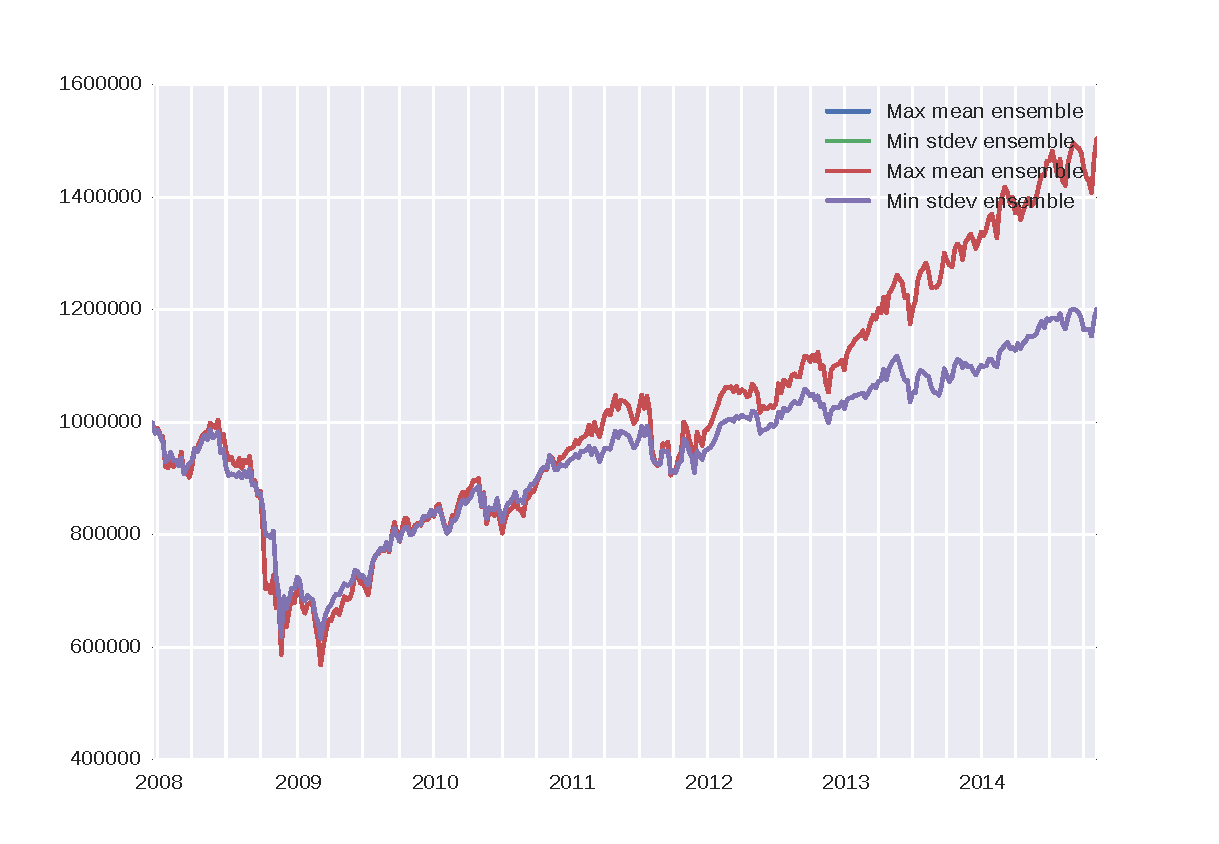
\includegraphics{../pic/returns_1overN_only.pdf}
\caption{DELETE ME IN FINAL:\ Returns for the 1/N strategy for the ensembles indicated.}
\label{fig:bondsyield}
\end{figure}
